% An extensibly causal quantum process with no purification.
% Physical Superintelligence (PSI), draft of 15 October 2026.
% Self-contained: no \input files. Compile with pdflatex (revtex4-2).
\documentclass[aps,prl,reprint,superscriptaddress,nofootinbib,longbibliography,raggedbottom]{revtex4-2}
\usepackage[T1]{fontenc}
\usepackage{amsmath,amssymb,amsthm}
\usepackage{newtxtext,newtxmath}
\usepackage{microtype}
\usepackage{xcolor}
\usepackage{tikz}
\usepackage[hidelinks]{hyperref}
\hypersetup{
  pdftitle={An extensibly causal quantum process with no purification},
  pdfauthor={David Turturean and Ning Bao}
}

\DeclareMathOperator{\Tr}{Tr}
\newcommand{\R}{\mathcal R}
\newcommand{\ket}[1]{\lvert #1\rangle}
\newcommand{\bra}[1]{\langle #1\rvert}
\newcommand{\proj}[1]{\ket{#1}\!\bra{#1}}
\newtheorem*{theorem*}{Theorem}
\newtheorem{lemma}{Lemma}
\newtheorem*{theoremA}{Theorem A}



\AtBeginDocument{\providecommand{\doi}{}\renewcommand{\doi}[1]{\href{https://doi.org/#1}{\nolinkurl{doi:#1}}}}
\begin{document}

\title{An extensibly causal quantum process with no purification}
\author{David Turturean}\thanks{D.T. built and ran the automated research and formalization workflows at PSI and steered the writing of the paper.}
\affiliation{Physical Superintelligence PBC, Cambridge, Massachusetts, USA}
\author{Ning Bao}\thanks{N.B. reviewed the manuscript and wrote a referee report, including improvements suggested by an AI review, as a paid contractor to PSI, not under one of his grants or as an employee of Northeastern University.}
\affiliation{Northeastern University}
\affiliation{Brookhaven National Laboratory}

\begin{abstract}
The process-matrix formalism describes two laboratories connected in a way
that does not presuppose which of them acts first. Two conditions have been
proposed to single out the ``physical'' processes. One is observational: a
process is extensibly causal if the statistics of every experiment, including
experiments assisted by arbitrary shared entanglement, can be explained by a
mixture of the two causal orders. The other is structural: a process is
purifiable if it is the restriction of a larger process that carries
reversible local operations to a reversible global evolution. Every
purifiable bipartite process is extensibly causal, and an open problem exists as to whether the converse holds. We show that the converse is false, by exhibiting
a process on four qubits that is extensibly causal
but not purifiable. 
\end{abstract}

\maketitle

{\raggedright\setlength{\parskip}{0.4\baselineskip}
\section*{Acknowledgements}

We thank Adam Levine for writing up and polishing the manuscript, Ian MacCormack for a verification package, and Jim Halverson for coordinating the expert review. We also thank Physical Superintelligence PBC, in which some of the authors have a financial interest, for use of its resources, including its technology and frontier AI models. The authors used these models to develop, derive, and compose this manuscript and its Lean~4 supplements.

Results were formalized in Lean~4 by AI agents and checked by Lean's kernel; the formalization is at \url{https://github.com/physical-superintelligence/oqp-batch-2026/tree/main/oqp43-extensible-causality/lean}.

David Turturean and Ning Bao reviewed and edited this paper and are responsible for its correctness. David Turturean is employed by PSI and has a financial interest in it.

\par}
\par\medskip\noindent\rule{\columnwidth}{0.4pt}\par\medskip


In ordinary quantum mechanics, an experiment involving two laboratories comes
with a causal structure: Alice acts before Bob, or Bob before Alice, or the
two are spacelike separated and neither can signal to the other. Oreshkov,
Costa, and Brukner \cite{OCB} asked what the most general way to connect two
laboratories is if one keeps the quantum formalism inside each laboratory
but gives up a global causal order. The answer is a process matrix: a positive operator $S$ that assigns
a probability to every pair of local operations, generalizing both a
bipartite state and a channel from one laboratory to the other. Surprisingly, some valid process matrices are not mixtures of the two
causal orders, and some of these produce correlations violating
``causal inequalities,'' the analog for causal order of Bell's inequalities
\cite{OCB,Branciard}.

No physical realization of such correlations is known, which raises the
question of what additional condition singles out the physical process
matrices. Two conditions have been proposed, and the purpose of
this Letter is to show that they are not equivalent. The first is a
condition on the probabilities that experiments produce. A process is \emph{causal} if the statistics of
every experiment performed on it can be explained as a mixture of ``Alice
acts first'' and ``Bob acts first,'' and it is \emph{extensibly causal} if
this remains true when the two laboratories are supplied with an arbitrary
shared ancilla, which may be entangled \cite{OG}. The second condition,
proposed by Ara\'ujo, Feix, Navascu\'es, and Brukner \cite{AFNB}, is a
condition on the process itself, modeled on two basic facts of ordinary
quantum mechanics: every mixed state is the marginal of a pure state, and
every channel is the restriction of a unitary evolution. A process is
\emph{purifiable} if it is the restriction of a larger process that is
reversible, in the sense that it maps reversible local operations to a
reversible global evolution. A third notion sits between these two. A
process is \emph{causally separable} if it is itself a mixture of an
Alice-first process and a Bob-first process. Such a process is clearly
extensibly causal. It is also purifiable, by purifying each
ordered component and letting a control qubit choose between them; and
conversely, a theorem of Refs.~\cite{YQSM,BLO} states that every purifiable
bipartite process is causally separable. So for two laboratories the first
two notions coincide, and the logical picture is that of
Fig.~\ref{fig:nesting}. Problem~43 of the IQOQI list of open problems in
quantum information asks whether the picture collapses further: whether
every extensibly causal process is purifiable \cite{OQP}.

\begin{figure}[t]
\centering
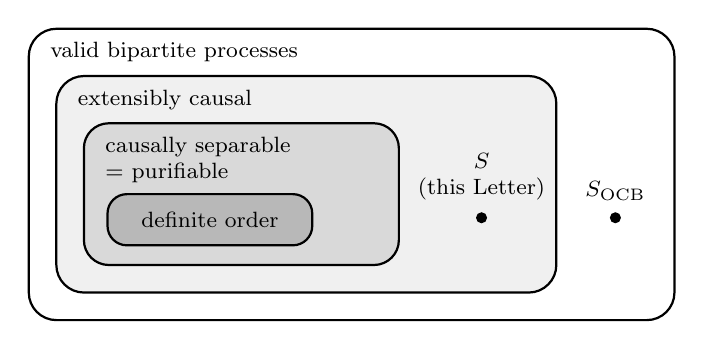
\begin{tikzpicture}[x=1cm,y=1cm,font=\footnotesize]
\draw[rounded corners=10pt,thick] (0,0) rectangle (8.2,3.7);
\node[anchor=north west] at (0.15,3.65) {valid bipartite processes};
\draw[rounded corners=10pt,thick,fill=black!6] (0.35,0.35) rectangle (6.7,3.1);
\node[anchor=north west] at (0.5,3.05) {extensibly causal};
\draw[rounded corners=9pt,thick,fill=black!15] (0.7,0.7) rectangle (4.7,2.5);
\node[anchor=north west,align=left] at (0.85,2.45)
  {causally separable\\ $=$ purifiable};
\draw[rounded corners=7pt,thick,fill=black!28] (1.0,0.95) rectangle (3.6,1.6);
\node at (2.3,1.275) {definite order};
\fill (5.75,1.3) circle (2pt);
\node[above,align=center] at (5.75,1.4) {$S$\\ (this Letter)};
\fill (7.45,1.3) circle (2pt);
\node[above] at (7.45,1.4) {$S_{\rm OCB}$};
\end{tikzpicture}
\caption{Nesting of the three properties for a bipartite process with
trivial global past and future. Purifiability and causal separability
coincide and lie strictly inside extensible causality; the process $S$
constructed here lies in the gap. The process $S_{\rm OCB}$ of
Ref.~\cite{OCB} violates a causal inequality and lies outside all three.}
\label{fig:nesting}
\end{figure}

We will show that the answer is no: there is a process on four qubits, which is extensibly causal but not purifiable. The
idea is simple to state. For a causally separable process, one
decomposition of the operator explains all experiments at once, with the
same weight $\lambda$ in every experiment. Extensible causality asks for
less. It
requires only that the probability table of each experiment be some
mixture of an
Alice-first table and a Bob-first table; the two tables and the weight may
be chosen afresh for each experiment, and they need not be the statistics
of any process matrix. Our example lives in the gap between these two
requirements. Feix, Ara\'ujo, and Brukner \cite{FAB} showed that causally
nonseparable processes exist whose statistics are nevertheless causal in
every experiment without ancillas, and found numerical evidence that some
of them remain causal with entangled ancillas, but were unable to prove it;
the difficulty is to control arbitrary measurements on arbitrary ancillas
at once. The main new ingredient here is an
operator identity of sum-of-squares type that does precisely this.

\medskip
\section{Review of processes and causal order}
Consider an experiment in which Alice chooses a setting $x$ and records an
outcome $a$, while Bob chooses $y$ and records $b$. Whatever connects the
laboratories, all that is observed is the conditional distribution
$p(a,b|x,y)$. We call such a distribution \emph{causal} if
\begin{equation}\label{causal}
p=\lambda\,p^{A\prec B}+(1-\lambda)\,p^{B\prec A},\qquad 0\leq\lambda\leq1,
\end{equation}
where $p^{A\prec B}$ and $p^{B\prec A}$ are conditional distributions such
that Alice's marginal of $p^{A\prec B}$ does not depend on $y$, and Bob's
marginal of $p^{B\prec A}$ does not depend on $x$. Here $\lambda$ is a
single number, the same for all settings. The condition on $p^{A\prec B}$
only forbids signaling from Bob to Alice; Bob's outcome may depend on
Alice's setting. Causality is therefore a much weaker requirement than Bell
locality, which demands that
$p(a,b|x,y)=\sum_\mu q(\mu)\,p_A(a|x,\mu)\,p_B(b|y,\mu)$ for some classical
variable $\mu$ shared by the laboratories, and so forbids signaling in both
directions and more. A causal inequality is a linear inequality
satisfied by all causal distributions \cite{OCB,Branciard}.

Now let the laboratories be quantum. Alice's has an input Hilbert space
$A_I$ and an output space $A_O$, and Bob's has $B_I$ and $B_O$; all four
are finite dimensional, and in our example they are qubits. The most
general thing Alice can do is apply a quantum instrument: a family of
completely positive maps $\mathcal M_{a|x}$ from $A_I$ to $A_O$, labeled by
her setting $x$ and outcome $a$, whose sum over $a$ is trace preserving. We
represent $\mathcal M_{a|x}$ by its Choi matrix $M_{a|x}$, a positive
operator on $A_I\otimes A_O$ normalized so that
$\sum_a\Tr_{A_O}M_{a|x}=I_{A_I}$.\footnote{We use the convention of
\cite{OCB}, in which $M$ is the transpose of the usual Choi matrix
$\sum_{ij}\ket i\bra j\otimes\mathcal M(\ket i\bra j)$; nothing below
depends on this.} Bob's instrument is represented likewise by operators
$N_{b|y}$ on $B_I\otimes B_O$. A process matrix is an operator $S$ on
$A_I\otimes A_O\otimes B_I\otimes B_O$ such that
\begin{equation}\label{born}
p(a,b|x,y)=\Tr\bigl[S\,(M_{a|x}\otimes N_{b|y})\bigr]
\end{equation}
is a probability distribution for every pair of instruments. Thus
$S\geq0$, and $\Tr[S(M\otimes N)]=1$ whenever $M$ and $N$ are Choi matrices
of quantum channels (completely positive and trace-preserving maps).
The normalization condition amounts to linear
constraints on $S$, written out in \cite{OCB}, which forbid any term by
which a laboratory could influence its own input, or by which the two
laboratories influence each other simultaneously; we will verify them
directly for our example. A process $S$ is \emph{causal} if \eqref{born}
is causal for all instruments, and \emph{extensibly causal} \cite{OG} if,
moreover, $S\otimes\sigma$ is causal for every density matrix $\sigma$ on
any pair of ancillary spaces $R_A\otimes R_B$, where now Alice's
instruments act on $A_I\otimes R_A$ and Bob's on $B_I\otimes R_B$. Neither
the ancilla dimensions nor the number of settings and outcomes are
restricted, and the associated decomposition \eqref{causal} may depend on $\sigma$ and
on the whole collection of instruments. In other words, extensible
causality constrains $S$ only through its outputs: every table
$p(a,b|x,y)$ that $S$ can produce must admit some decomposition of the
form \eqref{causal}, and nothing is asked of the form of $S$ itself.

Two familiar process matrices will be needed. If
$S=\rho\otimes I_{A_O}\otimes I_{B_O}$
for a density matrix $\rho$ on $A_I\otimes B_I$ (tensor factors are always
understood in the order $A_I,A_O,B_I,B_O$), Alice and Bob measure a shared
state and their outputs are discarded; there is no signaling. If instead $S=\widehat S\otimes
I_{B_O}$ with $\widehat S\geq0$ on $A_I\otimes A_O\otimes B_I$ and
$\Tr_{B_I}\widehat S=\rho\otimes I_{A_O}$ for a density matrix $\rho$ on
$A_I$, then Alice receives the state $\rho$, her output is sent through a
channel to Bob's input, and Bob's output is discarded. This is the general
form of a process in which Alice acts before Bob \cite{CDP}; we say that
$S$ has order $A\prec B$. A valid $S$ has order $A\prec B$ precisely when
it does not depend on $B_O$, which we write as $S=\R_{B_O}S$, where for any
tensor factor $Y$ the ``replacement'' map is
$\R_Y(T)=\Tr_YT\otimes I_Y/\dim Y$. Likewise $S$ has order $B\prec A$
precisely when $S=\R_{A_O}S$. A process is \emph{causally separable} if it
is a convex combination
\begin{equation}\label{CS}
S=\lambda\,S^{A\prec B}+(1-\lambda)\,S^{B\prec A}
\end{equation}
of processes of the two orders. Such a process is causal in every
experiment, with or without ancillas, since the two terms of \eqref{CS}
produce the two terms of \eqref{causal} with the same $\lambda$. Thus, every causally separable process is extensibly causal. The converse is what we show to be false in this letter. 

\medskip
\begin{figure}[t]
\centering
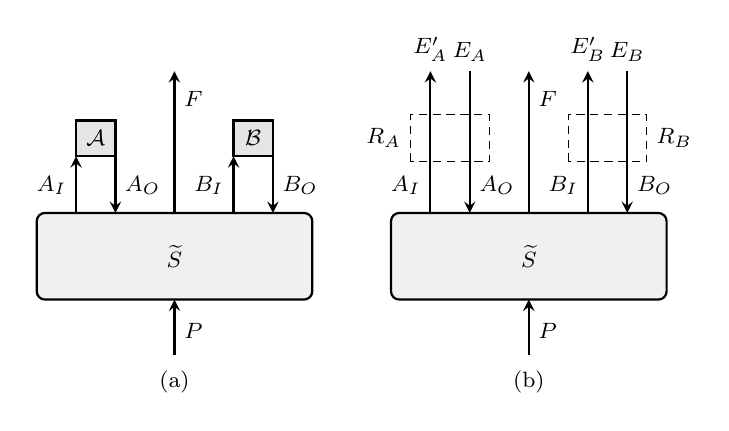
\begin{tikzpicture}[x=1cm,y=1cm,font=\footnotesize,>=stealth,
  wire/.style={thick,->},
  op/.style={draw,thick,fill=black!10,minimum width=5mm,minimum height=4.5mm,inner sep=1pt}]
\foreach \dx/\lab in {0/a,4.5/b} {
 \begin{scope}[xshift=\dx cm]
  \draw[thick,rounded corners=3pt,fill=black!6] (0,0) rectangle (3.5,1.1);
  \node at (1.75,0.55) {$\widetilde S$};
  \draw[wire] (1.75,-0.7) -- (1.75,0);
  \node[right] at (1.75,-0.4) {$P$};
  \draw[wire] (1.75,1.1) -- (1.75,2.9);
  \node[right] at (1.75,2.55) {$F$};
  \node at (1.75,-1.05) {(\lab)};
 \end{scope}
}
\node[op] at (0.75,2.05) {$\mathcal A$};
\draw[wire] (0.5,1.1) -- (0.5,1.82);
\node[left] at (0.5,1.45) {$A_I$};
\draw[wire] (1.0,1.82) -- (1.0,1.1);
\node[right] at (1.0,1.45) {$A_O$};
\node[op] at (2.75,2.05) {$\mathcal B$};
\draw[wire] (2.5,1.1) -- (2.5,1.82);
\node[left] at (2.5,1.45) {$B_I$};
\draw[wire] (3.0,1.82) -- (3.0,1.1);
\node[right] at (3.0,1.45) {$B_O$};
\begin{scope}[xshift=4.5cm]
  \draw[densely dashed] (0.25,1.75) rectangle (1.25,2.35);
  \node[left] at (0.25,2.05) {$R_A$};
  \draw[wire] (0.5,1.1) -- (0.5,2.9);
  \node[left] at (0.5,1.45) {$A_I$};
  \node[above] at (0.5,2.9) {$E'_A$};
  \draw[wire] (1.0,2.9) -- (1.0,1.1);
  \node[right] at (1.0,1.45) {$A_O$};
  \node[above] at (1.0,2.9) {$E_A$};
  \draw[densely dashed] (2.25,1.75) rectangle (3.25,2.35);
  \node[right] at (3.25,2.05) {$R_B$};
  \draw[wire] (2.5,1.1) -- (2.5,2.9);
  \node[left] at (2.5,1.45) {$B_I$};
  \node[above] at (2.5,2.9) {$E'_B$};
  \draw[wire] (3.0,2.9) -- (3.0,1.1);
  \node[right] at (3.0,1.45) {$B_O$};
  \node[above] at (3.0,2.9) {$E_B$};
\end{scope}
\end{tikzpicture}
\caption{(a) A process $\widetilde S$ with global past $P$, global future $F$, and
two laboratory slots: Alice's operation $\mathcal A$ receives $A_I$ and
returns $A_O$, and likewise Bob's. (b) With the swaps $R_A,R_B$ of
Eq.~\eqref{swap} inserted (dashed), each input is routed straight out to
$E'_A,E'_B$ and the external systems $E_A,E_B$ straight in. The map from
$P\otimes E_A\otimes E_B$ to $F\otimes E'_A\otimes E'_B$ is $\widetilde S$ itself with
its legs renamed, so purity makes $\widetilde S$ the Choi operator of a unitary,
Eq.~\eqref{rankone}.}
\label{fig:wires}
\end{figure}

\textit{Purification.---}%
Suppose that, besides the four laboratory spaces, a process has a global
past $P$ and a global future $F$. The process is then a positive operator $\widetilde S$ on
$P\otimes A_I\otimes A_O\otimes B_I\otimes B_O\otimes F$ with the property
that inserting channels in the two laboratories produces a channel from $P$
to $F$ \cite{CDP,AFNB}. Following \cite{AFNB}, we say that $\widetilde S$ is \emph{pure} if,
whenever the two local operations are unitary, the resulting map from $P$
to $F$ is unitary. The local unitaries may act also on auxiliary systems
passing through the laboratories, so purity concerns reversibility in all
circumstances. 

It is easy to show that a pure $\widetilde S$ also must be rank one. To see this, remember that the induced map
must be unitary for every choice of local unitaries, and so we may test it on a
choice. For example, let Alice apply the unitary that swaps her input
out to an external system $E'_A\cong A_I$ and an external system
$E_A\cong A_O$ in to her output,
\begin{equation}\label{swap}
R_A\,\ket i_{A_I}\ket o_{E_A}=\ket o_{A_O}\ket i_{E'_A},
\end{equation}
and let Bob apply $R_B$ likewise (Fig.~\ref{fig:wires}). Here and below,
for a linear map
$M\colon X\to Y$ we write $|M\rangle\!\rangle=\sum_k\ket k_X\otimes M\ket k$
for its Choi vector, so that $|M\rangle\!\rangle\langle\!\langle M|$ is the
Choi matrix of $\rho\mapsto M\rho M^\dagger$ and
$|I\rangle\!\rangle_{XY}=\sum_k\ket k_X\ket k_Y$. The Choi vector of the
swap is a pair of identity states,
$|I\rangle\!\rangle_{A_IE'_A}|I\rangle\!\rangle_{E_AA_O}$, and contracting
an index of $\widetilde S$ against one of them merely renames it. So the map induced from
$P\otimes E_A\otimes E_B$ to $F\otimes E'_A\otimes E'_B$ has Choi operator
$\widetilde S$ itself,
\begin{equation}\label{rankone}
\widetilde S=|\mathcal U\rangle\!\rangle\langle\!\langle\mathcal U|,\quad
\mathcal U\colon P\otimes A_O\otimes B_O\to A_I\otimes B_I\otimes F,
\end{equation}
with $\mathcal U$ unitary. The converse fails: a rank-one $\widetilde S$ only carries
unitary local operations to an isometry, which may enlarge the space, and
if that were allowed every process would be purifiable \cite{AFNB}. A
process $S$ with trivial past and future is \emph{purifiable} if it is
obtained
from a pure $\widetilde S$ by feeding a fixed state into the past and discarding the
future, $S=\Tr_F[\bra0_P\,\widetilde S\,\ket0_P]$, with $P$ and $F$ of arbitrary
finite dimension.

Processes with a definite causal order are purifiable, by the Stinespring
dilation of the circuit that realizes them \cite{CDP}. A mixture of processes as in
\eqref{CS} is also purifiable, by the mechanism of the quantum switch.
By \eqref{rankone}, write
$\widetilde S_A=|s_A\rangle\!\rangle\langle\!\langle s_A|$ and
$\widetilde S_B=|s_B\rangle\!\rangle\langle\!\langle s_B|$ for purifications of
$S^{A\prec B}$ and $S^{B\prec A}$, with pasts $P_A,P_B$ and futures
$F_A,F_B$, and let $|v_A\rangle\!\rangle$ on $P_A\otimes F_A$ be the vector
obtained from $|s_A\rangle\!\rangle$ by inserting identity operations in
both laboratories; it represents a unitary $V_A\colon P_A\to F_A$. Define
$|v_B\rangle\!\rangle$ likewise. Add a control qubit $C$ to the past and
$C'$ to the future, and set
\begin{equation}\label{switch}
\begin{split}
|s\rangle\!\rangle={}&
|\phi_0\rangle_C|0\rangle_{C'}\,|s_A\rangle\!\rangle|v_B\rangle\!\rangle\\
&+|\phi_1\rangle_C|1\rangle_{C'}\,|v_A\rangle\!\rangle|s_B\rangle\!\rangle,
\end{split}
\end{equation}
with $|\phi_0\rangle=\sqrt\lambda\ket0+\sqrt{1-\lambda}\ket1$\vadjust{\vskip1.5pt} and
$|\phi_1\rangle\perp|\phi_0\rangle$. Inserting unitary local operations
into $\widetilde S=|s\rangle\!\rangle\langle\!\langle s|$ gives the map
\begin{equation}\label{switchmap}
G=\ket0\bra{\phi_0}\otimes G_A\otimes V_B
 +\ket1\bra{\phi_1}\otimes V_A\otimes G_B ,
\end{equation}
where $G_A,G_B$ are the unitaries induced by $\widetilde S_A,\widetilde S_B$. So $G$ is unitary,
and $\widetilde S$ is pure (it maps channels to channels by the same block structure).
Feeding $\ket0$ into $C$ selects the amplitudes
$\langle0|\phi_0\rangle=\sqrt\lambda$ and
$\langle0|\phi_1\rangle=\sqrt{1-\lambda}$, and tracing out $F$ kills the
cross terms, the two branches being orthogonal on $C'$; since
$\langle0|V_B^\dagger V_B|0\rangle=1$, the result is
$\Tr_F[\bra0_PS\ket0_P]=\lambda S^{A\prec B}+(1-\lambda)S^{B\prec A}$, as
required. The converse is the theorem of Yokojima, Quintino, Soeda, and
Murao \cite{YQSM} and of Barrett, Lorenz, and Oreshkov \cite{BLO}:
\emph{a purifiable bipartite process with trivial past and future is
causally separable.} Its proof starts from \eqref{rankone} and shows that
the constraints forbidding each laboratory from influencing its own input
split $P$ into sectors, in each of which the order is definite;
discarding $F$ destroys the coherence between sectors, leaving a mixture
\eqref{CS}.

Thus, for two laboratories, purifiability and causal separability are the
same property, and it will suffice therefore to show that our extensibly causal process is not causally
separable. A convenient tool for that is a causal witness \cite{Witnesses}: a Hermitian operator $W$ with
$\Tr(WS')\geq0$ for every causally separable $S'$. A sufficient condition
is that $\R_{B_O}W\geq0$ and $\R_{A_O}W\geq0$, for if $S'$ has order
$A\prec B$ then
$\Tr(WS')=\Tr(W\,\R_{B_O}S')=\Tr[(\R_{B_O}W)\,S']\geq0$, the map
$\R_{B_O}$ being self-adjoint with respect to the trace pairing; similarly
for the other order, and then for mixtures.


\medskip
\section{A non-causally separable but extensibly causal process}\label{sec:main}
We now turn to explaining the counterexample in detail. We will find a causally separable witness $W$ and an extensibly causal process with operator $S$ such that
\begin{align}
\Tr(SW)\leq0.
\end{align}


Let $I$, $X$, $Z$ be the identity and Pauli matrices on a qubit, and let
a string of four Paulis denote the tensor product in the order $A_IA_OB_IB_O$ (i.e.\ $X \otimes X \otimes I \otimes Z$ is denoted by $XXIZ$). Our
process is
\begin{equation}\label{W}
\begin{split}
S=\frac1{80}\bigl(&20\,IIII+10\,ZIII+10\,IIZI\\
&+5\,ZIZI+4\,IZZI+4\,ZIXZ\bigr).
\end{split}
\end{equation}
Compare the process
$S_{\rm OCB}=\frac14\bigl[IIII+(IZZI+ZIXZ)/\sqrt2\bigr]$ of \cite{OCB},
which violates a causal inequality. The last two terms of \eqref{W} are the
signaling terms of $S_{\rm OCB}$: $IZZI$ sends Alice's output, in the $Z$
basis, to Bob's input, and $ZIXZ$ sends Bob's output to Alice's input,
conditioned on the $X$ component of Bob's input. Here they carry the
smaller coefficient $1/20$, and the first
four terms, which add up to $\theta\otimes I\otimes\theta\otimes I$ with
$\theta=\frac14(3\proj0+\proj1)$, describe a biased rather than maximally
mixed state on the inputs. The bias is essential to the argument below. To our knowledge $S$ has not been considered before. The nonseparable
processes with causal models of Ref.~\cite{FAB} are built instead from a
depolarizing channel and $ZIXZ$, and their causal models rest on a
partial-transposition argument that neither extends to entangled ancillas
nor applies to $S$, which is invariant under partial transposition of
Bob's systems.

\begin{theorem*}
The operator $S$ of \eqref{W} is a valid process matrix of full rank. It is
extensibly causal, but is not causally separable. Consequently it has no
purification, whatever the dimensions of $P$ and $F$.
\end{theorem*}

First we check that $S$ is a valid process matrix. Let $M$ and $N$ be Choi
matrices of channels, so that $\Tr_{A_O}M=I$ and $\Tr_{B_O}N=I$. The term
$IZZI$ contributes $\Tr[(IZ)_{A_I \otimes A_O}M]\,\allowbreak\Tr[(ZI)_{B_I \otimes B_O}N]$, and the second factor is
$\Tr[Z\,\Tr_{B_O}N]=\Tr Z=0$; the term $ZIXZ$ contributes zero for the same
reason, with the roles of the laboratories exchanged. The first four terms
contribute $\Tr[\theta\Tr_{A_O}M]\,\Tr[\theta\Tr_{B_O}N]=1$. The same
computation applies to $S\otimes\sigma$ in the presence of ancillas. For
positivity, every term in \eqref{W} is diagonal in the computational basis
except the $X$ in the last one, so $S$ is a direct sum of $2\times2$ blocks
on $B_I$. Up to the sign of the
off-diagonal entry, the blocks of $80S$ are
\begin{equation}\label{blocks}
\begin{pmatrix}49&4\\4&11\end{pmatrix},\ \
\begin{pmatrix}41&4\\4&19\end{pmatrix},\ \
\begin{pmatrix}19&4\\4&1\end{pmatrix},\ \
\begin{pmatrix}11&4\\4&9\end{pmatrix},
\end{equation}
with determinants $523$, $763$, $3$, and $83$. So $S>0$, with smallest
eigenvalue $(10-\sqrt{97})/80\approx0.0019$.

\medskip
\subsection*{$S$ is not causally separable}
A simple calculation shows that $S$ is not causally separable. Let $P_1=\proj1$ and $D=I+8P_1=\mathrm{diag}(1,9)$, and set
\begin{equation}\label{Sw}
W=P_1\,I\,D\,I-P_1\,Z\,(DZ)\,I+3\,P_1\,I\,X\,Z .
\end{equation}
We claim that $W$ is a causal witness. Applying $\R_{B_O}$ kills the
last term and leaves $P_1\otimes(I\otimes D-Z\otimes DZ)\otimes I$. On the
two eigenspaces of $Z$ on $A_O$, the operator on $B_I$ is $D(I\mp Z)$, that
is, $18P_1$ or $2\proj0$; both are positive. Applying $\R_{A_O}$ instead
kills the middle term and leaves
$P_1\otimes I\otimes(D\otimes I+3X\otimes Z)$. On the two eigenspaces of
$Z$ on $B_O$, the operator on $B_I$ is
$D\pm3X=\bigl(\begin{smallmatrix}1&\pm3\\\pm3&9\end{smallmatrix}\bigr)$,
which is positive and of rank one. On the other hand, writing
$P_1=(I-Z)/2$ and $D=5I-4Z$ and using the orthogonality of distinct Pauli
strings, one finds that
the three terms of \eqref{Sw} contribute $3$, $-2$, and $-6/5$ to
$\Tr(WS)$, so that
\begin{equation}\label{negative}
\Tr(WS)=-\tfrac15<0 .
\end{equation}
Thus $S$ is not causally separable, and by the theorem of \cite{YQSM,BLO}
it is not purifiable. Note that \eqref{negative} concerns the operator $S$;
it does not say that $S$ violates a causal inequality, and we now show that
it violates none, even with entangled ancillas.

\medskip
\subsection*{$S$ is extensibly causal}
Now we demonstrate that $S$ is in fact extensibly causal. The argument has
two steps: a general criterion, Lemma~\ref{lem:flow}, which guarantees extensible causality of the process, and the verification, Lemma~\ref{lem:bound}, that $S$ meets this
criterion in every experiment.

\begin{lemma}\label{lem:flow}
Let $S$ be a bipartite process and $\lambda\in(0,1)$. Suppose that for
every ancilla state $\sigma$ and every pair of instruments there are
nonnegative numbers $r_A(a|x)$ and $r_B(b|y)$, the first depending only on
$x$ and the second only on $y$, with $\sum_ar_A(a|x)=\lambda$ and
$\sum_br_B(b|y)=1-\lambda$, such that for all sets $\alpha$ of Alice's
outcomes and $\beta$ of Bob's outcomes
\begin{equation}\label{rectangle}
p(\alpha,\beta|x,y)\leq r_A(\alpha|x)+r_B(\beta|y),
\end{equation}
with sums over $a\in\alpha$ and $b\in\beta$ being understood. Then $S$ is
extensibly causal.
\end{lemma}

\begin{figure}[t]
\centering
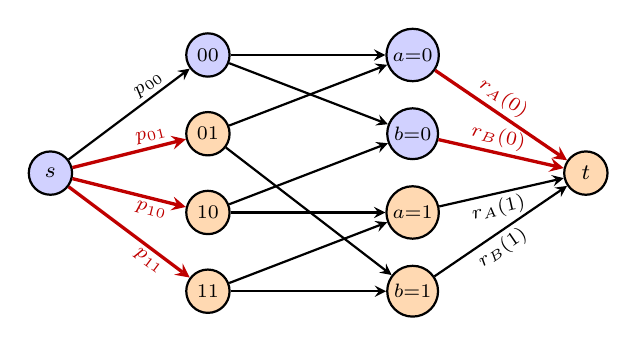
\begin{tikzpicture}[x=1cm,y=1cm,font=\footnotesize,>=stealth,
  src/.style={draw,thick,circle,fill=blue!18,inner sep=1.5pt,minimum size=5.5mm},
  snk/.style={draw,thick,circle,fill=orange!30,inner sep=1.5pt,minimum size=5.5mm},
  pipe/.style={thick,->},
  cutpipe/.style={very thick,->,red!75!black},
  lab/.style={font=\scriptsize,inner sep=1.5pt}]
\node[src] (s) at (0,0) {$s$};
\node[src] (c00) at (2.0,1.5) {\scriptsize$00$};
\node[snk] (c01) at (2.0,0.5) {\scriptsize$01$};
\node[snk] (c10) at (2.0,-0.5) {\scriptsize$10$};
\node[snk] (c11) at (2.0,-1.5) {\scriptsize$11$};
\node[src] (a0) at (4.6,1.5) {\scriptsize$a{=}0$};
\node[src] (b0) at (4.6,0.5) {\scriptsize$b{=}0$};
\node[snk] (a1) at (4.6,-0.5) {\scriptsize$a{=}1$};
\node[snk] (b1) at (4.6,-1.5) {\scriptsize$b{=}1$};
\node[snk] (t) at (6.8,0) {$t$};
\draw[pipe] (s) -- node[lab,pos=0.72,sloped,above] {$p_{00}$} (c00);
\draw[cutpipe] (s) -- node[lab,pos=0.72,sloped,above] {$p_{01}$} (c01);
\draw[cutpipe] (s) -- node[lab,pos=0.72,sloped,below] {$p_{10}$} (c10);
\draw[cutpipe] (s) -- node[lab,pos=0.72,sloped,below] {$p_{11}$} (c11);
\draw[pipe] (c00) -- (a0); \draw[pipe] (c00) -- (b0);
\draw[pipe] (c01) -- (a0); \draw[pipe] (c01) -- (b1);
\draw[pipe] (c10) -- (a1); \draw[pipe] (c10) -- (b0);
\draw[pipe] (c11) -- (a1); \draw[pipe] (c11) -- (b1);
\draw[cutpipe] (a0) -- node[lab,pos=0.45,sloped,above] {$r_A(0)$} (t);
\draw[cutpipe] (b0) -- node[lab,pos=0.45,sloped,above] {$r_B(0)$} (t);
\draw[pipe] (a1) -- node[lab,pos=0.45,sloped,below] {$r_A(1)$} (t);
\draw[pipe] (b1) -- node[lab,pos=0.45,sloped,below] {$r_B(1)$} (t);
\end{tikzpicture}
\caption{The network behind Eq.~\eqref{transport}, drawn for two outcomes
per party. Fluid enters at the source $s$, reaches the outcome nodes
through pipes of capacity $p_{ab}$, flows on through pipes of unlimited
capacity to the row node $a$ and the column node $b$ of each outcome, and
leaves through pipes of capacity $r_A(a|x)$, $r_B(b|y)$ into the sink $t$.
A division \eqref{transport} is a way of sending one unit through this
network. The colors show the cut with $\alpha=\beta=\{0\}$: blue nodes
($s$, the outcome $00$, and the row and column nodes in $\alpha$ and
$\beta$) are those still connected to the source after the cut, orange
nodes are those cut off. The removed pipes, in red, are exactly the ones
running from a blue node to an orange node, $s\to01$, $s\to10$, $s\to11$,
$a{=}0\to t$ and $b{=}0\to t$, of total capacity
$r_A(0|x)+r_B(0|y)+1-p_{00}$, which Eq.~\eqref{rectangle} makes at least
one. Pipes from orange to blue nodes are not removed.}
\label{fig:flow}
\end{figure}
\begin{proof}
Fix an experiment and settings $x,y$, and write $p_{ab}$ for
$p(a,b|x,y)$. We want to divide the probability $p_{ab}$ of each outcome
$(a,b)$ into a part $z_{ab}$ credited to Alice's outcome $a$ and a
remainder $p_{ab}-z_{ab}$ credited to Bob's outcome $b$, such that the
total credited to each $a$ is $r_A(a|x)$ and the total credited to each
$b$ is $r_B(b|y)$:
\begin{equation}\label{transport}
\begin{gathered}
0\leq z_{ab}\leq p_{ab},\\
\sum_b z_{ab}=r_A(a|x),\qquad \sum_a(p_{ab}-z_{ab})=r_B(b|y).
\end{gathered}
\end{equation}
The totals are consistent, since
$\sum_{ab}p_{ab}=1=\sum_ar_A(a|x)+\sum_br_B(b|y)$. Whether such a division
exists can be recast as a question about pipes (Fig.~\ref{fig:flow}).
Picture a source connected to one node per outcome $(a,b)$ by a pipe of
capacity $p_{ab}$. Connect each outcome node by pipes of unlimited capacity
to a node for its row $a$ and a node for its column $b$ (as illustrated in Fig.~\ref{fig:flow}). Furthermore, connect each row node
$a$ and column node $b$ to a sink by pipes of capacity
$r_A(a|x)$ and $r_B(b|y)$. 

A \emph{flow} assigns to each pipe an amount of fluid between zero and
its capacity, such that at every node other than the source and the sink
the fluid entering equals the fluid leaving; the \emph{value} of the flow is the total
amount leaving the source node. It is not hard to see that a flow of value one is the same thing as a
division as in \eqref{transport}. The source pipes have total capacity
$\sum_{ab}p_{ab}=1$, so a flow of value one fills each of them exactly and
delivers $p_{ab}$ to the node $(a,b)$. Conservation at that node means it
passes some amount $z_{ab}\in[0,p_{ab}]$ on to its row node and the
remainder $p_{ab}-z_{ab}$ to its column node. Conservation at the row node
$a$ means that the pipe from $a$ to the sink carries $\sum_bz_{ab}$, which
cannot exceed its capacity $r_A(a|x)$; likewise
$\sum_a(p_{ab}-z_{ab})\leq r_B(b|y)$. Finally, the sink pipes must carry
one unit in total while their capacities add up to
$\sum_ar_A(a|x)+\sum_br_B(b|y)=1$, so in fact these inequalities are all
equalities. In other words, $z_{ab}$ must obey the equations in \eqref{transport}.

To show that the network can support a flow of value one, we use the
max-flow min-cut theorem together with the inequality \eqref{rectangle}.
A \emph{cut} is a division of the nodes into a source side containing $s$
and a sink side containing $t$ (blue and orange in Fig.~\ref{fig:flow}),
and its capacity is the total capacity of the pipes leading from the
source side to the sink side; pipes in the other direction do not count.
Every unit of fluid that reaches $t$ must cross from the source side to
the sink side, so no flow has value larger than the capacity of any cut.
The max-flow min-cut theorem \cite{FordFulkerson} says that the largest
flow value through the network is exactly the smallest cut capacity.
Hence a flow of value one exists if and only if every cut has capacity at
least one, and it remains to list the cuts. Since the intermediate pipes
have infinite capacity, a cut of finite capacity never has an outcome node
on the source side while its row node or column node is on the sink side.
Let $\alpha$ be the set of rows and $\beta$ the set of columns on the
source side. An outcome $(a,b)$ with $a\notin\alpha$ or $b\notin\beta$,
that is, with $(a,b)\notin\alpha\times\beta$, must then be on the sink
side, so its source pipe crosses the cut; and the sink pipes of the rows in
$\alpha$ and the columns in $\beta$ cross it too. The capacity is
therefore at least
\begin{equation}\label{cut}
r_A(\alpha|x)+r_B(\beta|y)+\bigl[1-p(\alpha,\beta|x,y)\bigr],
\end{equation}
the bracket being the total capacity of the source pipes of the outcomes
outside $\alpha\times\beta$, with equality when every outcome of
$\alpha\times\beta$ is on the source side, as in Fig.~\ref{fig:flow}.
That \eqref{cut} is always at least one is exactly the inequality
\eqref{rectangle}; the value one is attained by the cut with only $s$ on
the source side ($\alpha=\beta=\emptyset$), whose capacity is
$\sum_{ab}p_{ab}=1$. Therefore the minimum cut capacity is one, a flow of
value one exists, and the division \eqref{transport} follows. 

Given this division $z_{ab}$, set $p^{A\prec B}=z/\lambda$ and
$p^{B\prec A}=(p-z)/(1-\lambda)$. These are normalized distributions with
$p=\lambda\,p^{A\prec B}+(1-\lambda)\,p^{B\prec A}$; Alice's marginal of
$p^{A\prec B}$ is $r_A(a|x)/\lambda$, independent of $y$, and Bob's
marginal of $p^{B\prec A}$ is $r_B(b|y)/(1-\lambda)$, independent of $x$.
The weight $\lambda$ and these marginals are the same for all settings, as
\eqref{causal} requires, so the table is causal. The experiment being
arbitrary, it follows that $S$ is extensibly causal.
\end{proof}

To apply the lemma to our $S$ we need one more ingredient, a decomposition
of $S$ that is almost, but not quite, of the form \eqref{CS}. Write
\begin{equation}\label{UVC}
\begin{gathered}
U=\tfrac1{20}(IIII+IZZI),\qquad V=\tfrac1{20}(IIII+ZIXZ),\\
C=\tfrac1{160}\,\mathrm{diag}(37,\,7,\,7,\,-3)\ \ \text{on }A_I\otimes B_I,
\end{gathered}
\end{equation}
and $Q_C=C\otimes I_{A_O}\otimes I_{B_O}$. Since the first four terms of
\eqref{W} are $\theta\otimes\theta$ on the inputs and
$\theta\otimes\theta=2C+\tfrac1{10}I\otimes I$,
\begin{equation}\label{signed}
S=U+V+2Q_C .
\end{equation}
Here $U\geq0$ has order $A\prec B$ and $V\geq0$ has order $B\prec A$, so
\eqref{signed} would be a causal decomposition if $C$ were positive. It is
not, but its negativity is mild: both marginals of $C$ equal
$\tfrac1{160}\,\mathrm{diag}(44,4)\geq0$, and this, together with the
identity \eqref{SOS} below, is all we use.

\begin{lemma}\label{lem:bound}
Let $S$ be the process \eqref{W}. For every ancilla state $\sigma$ on
$R_A\otimes R_B$ and every pair of instruments, with Choi matrices
$M_{a|x}$ on $A_I\otimes R_A\otimes A_O$ and $N_{b|y}$ on
$B_I\otimes R_B\otimes B_O$, the numbers
\begin{equation}\label{r}
\begin{gathered}
r_A(a|x)=\Tr\bigl[(\tfrac12\theta\otimes\sigma_{R_A})\,E_{a|x}\bigr],\\
r_B(b|y)=\Tr\bigl[(\tfrac12\theta\otimes\sigma_{R_B})\,H_{b|y}\bigr],
\end{gathered}
\end{equation}
with $E_{a|x}=\Tr_{A_O}M_{a|x}$, $H_{b|y}=\Tr_{B_O}N_{b|y}$,
$\sigma_{R_A}=\Tr_{R_B}\sigma$ and $\sigma_{R_B}=\Tr_{R_A}\sigma$, satisfy
the hypotheses of Lemma~\ref{lem:flow} with $\lambda=\tfrac12$.
\end{lemma}

\begin{proof}
The operators $E_{a|x}$ on $A_I\otimes R_A$ and $H_{b|y}$ on
$B_I\otimes R_B$ are the measurement operators that give the outcome
probabilities when the outputs are ignored; they are positive and sum to
the identity over outcomes. Hence $r_A\geq0$ depends only on $x$,
$r_B\geq0$ only on $y$, and each sums to $1/2$. It remains to prove
\eqref{rectangle}. Fix $\alpha,\beta$, let
$M=\sum_{a\in\alpha}M_{a|x}$ and $N=\sum_{b\in\beta}N_{b|y}$, with
$E=\Tr_{A_O}M$ on $A_I\otimes R_A$ and $H=\Tr_{B_O}N$ on $B_I\otimes R_B$,
so that $0\leq E,H\leq I$. Three facts are needed. First, the Born rule
\eqref{born} for the extended process $S\otimes\sigma$, with
\eqref{signed} inserted, splits into three terms,
\begin{equation}\label{bornext}
p(\alpha,\beta|x,y)=p_U+p_V+2\Tr\bigl[(C\otimes\sigma)(E\otimes H)\bigr],
\end{equation}
where $p_U=\Tr[(U\otimes\sigma)(M\otimes N)]$, $p_V$ is defined likewise,
and in the $Q_C$ term the identity on the outputs has traced $M$ and $N$
down to $E$ and $H$, so that this term is a trace over
$A_I\otimes B_I\otimes R_A\otimes R_B$. Second, since $U$ has order
$A\prec B$, the joint probability $p_U$ is at most the probability of
Alice's event alone, and similarly for $V$:
\begin{equation}\label{pU}
p_U\leq\Tr\bigl[(\tfrac1{10}I\otimes\sigma_{R_A})E\bigr],\quad
p_V\leq\Tr\bigl[(\tfrac1{10}I\otimes\sigma_{R_B})H\bigr].
\end{equation}
Here $\tfrac1{10}I$ is Alice's input state in $U$: replacing $N$ by the
full channel $\sum_bN_{b|y}\geq N$ can only increase $p_U$, and then
$\Tr_{B_O}\sum_bN_{b|y}=I$ and $\Tr_{B_I}\tfrac1{20}(III+IZZ)=\tfrac1{10}II$
give the stated value. Third, the reference marginals were built to
contain exactly these bounds: since
$\tfrac12\theta=\tfrac1{10}I+\Tr_{B_I}C$, definition \eqref{r} gives
\begin{equation}\label{rsplit}
\begin{split}
r_A(\alpha|x)&=\Tr\bigl[(\tfrac1{10}I\otimes\sigma_{R_A})E\bigr]
 +\Tr\bigl[(C\otimes\sigma)(E\otimes1)\bigr],\\
r_B(\beta|y)&=\Tr\bigl[(\tfrac1{10}I\otimes\sigma_{R_B})H\bigr]
 +\Tr\bigl[(C\otimes\sigma)(1\otimes H)\bigr].
\end{split}
\end{equation}
Combining these equations gives the inequality
\begin{equation}\label{slack}
\begin{split}
&r_A(\alpha|x)+r_B(\beta|y)-p(\alpha,\beta|x,y)\\
&\quad\geq\Tr\bigl[(C\otimes\sigma)(E\otimes1+1\otimes H-2E\otimes H)\bigr].
\end{split}
\end{equation}
The ordered parts $U,V$ of $S$ have dropped out entirely; only the signed
part $C$ remains to be controlled.
As $C$ is diagonal in the computational basis $\ket{ij}$ of $A_I\otimes B_I$,
only the blocks $E_i=\bra iE\ket i$, operators on $R_A$, and
$H_j=\bra jH\ket j$, operators on $R_B$, enter, and the right side is
$\tfrac1{160}\Tr[\sigma\,(37D_{00}+7D_{01}+7D_{10}-3D_{11})]$, a trace
over $R_A\otimes R_B$, with
$D_{ij}=E_i\otimes1+1\otimes H_j-2E_i\otimes H_j$. The $E_i,H_j$ are
arbitrary operators with $0\leq E_i,H_j\leq1$ on the ancillas $R_A,R_B$,
which have arbitrary dimension, and $E_0,E_1$ need not commute.
Nevertheless, with $L=7E_0+E_1-7H_0-H_1$ and $M=-E_0+E_1-H_0+H_1$,
\begin{equation}\label{SOS}
\begin{split}
37D_{00}&+7D_{01}+7D_{10}-3D_{11}\\
&=16(E_0-H_0)^2+\tfrac12L^2+\tfrac72M^2\\
&\quad+44\bigl[(E_0-E_0^2)+(H_0-H_0^2)\bigr]\\
&\quad+4\bigl[(E_1-E_1^2)+(H_1-H_1^2)\bigr],
\end{split}
\end{equation}
an identity between operators on $R_A\otimes R_B$ verified by expansion,
the cross terms $E_0E_1+E_1E_0$ and $H_0H_1+H_1H_0$ cancelling between
$L^2$ and $M^2$. Each square is positive and $E-E^2\geq0$ whenever
$0\leq E\leq1$, so the right side of \eqref{slack} is nonnegative and
\eqref{rectangle} holds.
\end{proof}

Lemmas~\ref{lem:flow} and~\ref{lem:bound} together show that $S$ is
extensibly causal, which completes the proof of the theorem. Nothing here is special to qubits: for any dimensions of the four spaces,
all at least two, there is an open set of extensibly causal nonpurifiable
processes, while if any space is one-dimensional every valid process is
ordered and purifiable. The proof, which reuses Lemmas~\ref{lem:flow} and~\ref{lem:bound}, is given in
Appendix~\ref{app:general}.

\medskip
\section{Discussion}
We have exhibited a bipartite process whose every experiment, with or
without shared entanglement, admits a causal explanation, and which
nevertheless has no purification. This answers Problem 43 in the negative,
in its finite-dimensional bipartite form and with the notion of purity of
\cite{AFNB}, and confirms the conjecture of \cite{FAB} that causally nonseparable bipartite processes exist which
remain causal under all entangled extensions. The lesson, we think, is that
extensible causality and purifiability test different things: the former
lets the causal explanation depend on the experiment, as \eqref{r} and
\eqref{transport} do through $\sigma$ and the instruments, whereas the
latter demands one explanation for all experiments, a decomposition of $S$
itself. We do not claim that $S$ is unphysical in every sense, only that
the purification postulate is strictly stronger than the absence of
causal-inequality violations.

\appendix
\setcounter{secnumdepth}{1}
\setcounter{equation}{0}
\renewcommand{\theequation}{A\arabic{equation}}
\section{General port dimensions, robustness, and the dimension boundary}
\label{app:general}

Write $(m,d,n,e)=(\dim A_I,\dim A_O,\dim B_I,\dim B_O)$. For the
robustness statement we need the linear constraints behind normalization
explicitly. A Hermitian $T$ on $A_I\otimes A_O\otimes B_I\otimes B_O$
satisfies $\Tr[T(M\otimes N)]=\Tr T/(de)$ for all pairs of channels if and
only if \cite{OCB,Witnesses}
\begin{equation}\label{A:LV}
\begin{gathered}
(1-\R_{A_O})\R_{B_IB_O}T=0,\qquad (1-\R_{B_O})\R_{A_IA_O}T=0,\\
(1-\R_{A_O})(1-\R_{B_O})T=0,
\end{gathered}
\end{equation}
with the replacement maps $\R_Y$ of the main text. Call the real space of
such $T$ $\mathcal L_V$; a valid process is $T\in\mathcal L_V$ with
$T\geq0$ and $\Tr T=de$. Replacement maps on different factors commute,
preserve $\mathcal L_V$ and the trace, and are positive and unital, hence
contractive in operator norm on Hermitian operators.

Now let $m,d,n,e\geq2$. In each space single out two basis vectors
$\ket0,\ket1$ and define, for $r\in\{m,d,n,e\}$,
\begin{equation}\label{A:local}
\begin{gathered}
P_r=\proj0+\proj1,\qquad Z_r=\proj0-\proj1,\\
X_r=\ket0\bra1+\ket1\bra0,\qquad Z_r^+=I_r-2\proj1,\\
\theta_r=\tfrac14\bigl(3\proj0+\proj1\bigr),
\end{gathered}
\end{equation}
so that $Z_r$ lives on the two distinguished vectors while $Z_r^+$ is an
involution on the whole space. Put $\Pi=P_m\otimes I_d\otimes P_n\otimes
I_e$, $G_A=P_m\otimes Z_d^+\otimes Z_n\otimes I_e$,
$G_B=Z_m\otimes I_d\otimes X_n\otimes Z_e^+$, and
\begin{equation}\label{A:S}
\begin{gathered}
\bar S=\theta_m\otimes I_d\otimes\theta_n\otimes I_e+\tfrac1{20}(G_A+G_B),\\
\bar S_{\rm c}=\tfrac{99}{100}\bar S+\tfrac1{100}\,\frac{I}{mn}.
\end{gathered}
\end{equation}
For four qubits $\bar S$ is the process \eqref{W}.

\begin{theoremA}
(a) For all $m,d,n,e\geq2$, $\bar S$ is a valid process of rank $4de$
that is extensibly causal and not causally separable. (b) Every
$\bar S_{\rm c}+H$ with $H\in\mathcal L_V$, $\Tr H=0$ and
$\|H\|_\infty\leq1/(300mn)$ is a full-rank extensibly causal process that
is not causally separable. (c) If $\min\{m,d,n,e\}=1$, every valid
process has a definite causal order and is purifiable.
\end{theoremA}
By the theorem of Refs.~\cite{YQSM,BLO}, ``not causally separable'' may be
read as ``not purifiable'' in (a) and (b). Hence, on a given port tuple,
every extensibly causal process is purifiable if and only if
$\min\{m,d,n,e\}=1$.

\emph{Proof of (a).} Validity is checked as in the main text: with
$\Tr_{A_O}M=I$ and $\Tr_{B_O}N=I$, the term $G_A$ contributes
$\Tr[(P_m\otimes Z_d^+)M]\,\Tr Z_n=0$, the term $G_B$ contributes zero by
$\Tr Z_m=0$, and the first term contributes $\Tr\theta_m\Tr\theta_n=1$.
The operator $\bar S$ vanishes outside the range of $\Pi$, which has
dimension $4de$, and on it, in a basis of eigenvectors of $Z_d^+$ and
$Z_e^+$, it is a direct sum of the $2\times2$ blocks \eqref{blocks} acting
on the two distinguished vectors of $B_I$; so $\bar S\geq0$ with rank
$4de$.

Lemma~\ref{lem:flow} is dimension-free. Lemma~\ref{lem:bound} and its
proof go through verbatim with $U=\tfrac1{20}(\Pi+G_A)$,
$V=\tfrac1{20}(\Pi+G_B)$, the same $C$, now a diagonal operator on
$A_I\otimes B_I$ supported on the four vectors $\ket{ij}$ with
$i,j\in\{0,1\}$, and $\theta_m,\theta_n$ in place of $\theta$ in
\eqref{r}. Indeed, the only facts about the qubit case that the proof used
were $S=U+V+2Q_C$, which holds for $\bar S$ because
$\theta_m\otimes\theta_n=2C+\tfrac1{10}P_m\otimes P_n$; that $U,V\geq0$
have orders $A\prec B$ and $B\prec A$, which holds because
$G_A^2=G_B^2=\Pi$ with both supported on the range of $\Pi$; the marginal
$\Tr_{B_I}\tfrac1{20}(P_m\otimes I_d\otimes P_n+P_m\otimes Z_d^+\otimes
Z_n)=\tfrac1{10}P_m\otimes I_d$, which replaces
$\tfrac1{10}I\otimes I$ in \eqref{pU}; the identity
$\tfrac12\theta_m=\tfrac1{10}P_m+\Tr_{B_I}C$; and the fact that only the
blocks $\bra iE\ket i$, $\bra jH\ket j$ with $i,j\in\{0,1\}$ enter the
$C$ term, so that the identity \eqref{SOS} applies unchanged. Hence
$\bar S$ is extensibly causal.

For nonseparability let $P_1=\proj1$ on $A_I$ and $D_n=I_n+8\proj1$ on
$B_I$, and take
\begin{equation}\label{A:W}
\begin{split}
\bar W={}&P_1\otimes P_d\otimes D_n\otimes P_e
 -P_1\otimes Z_d\otimes D_nZ_n^+\otimes P_e\\
&+3\,P_1\otimes P_d\otimes X_n\otimes Z_e ,
\end{split}
\end{equation}
which reduces to \eqref{Sw} for qubits. Applying $\R_{B_O}$ kills the last
term, and on the eigenspaces of $Z_d$ the operator on $B_I$ is
$D_n(I_n\mp Z_n^+)$, equal to $18\proj1$ or $2(I_n-\proj1)$, both
positive. Applying $\R_{A_O}$ kills the middle term, and on the eigenspaces
of $Z_e$ the operator on $B_I$ is $D_n\pm3X_n$, whose restriction to the
distinguished vectors is the rank-one positive matrix of the main text and
whose remainder is the identity. So $\bar W$ is a causal witness, and the
three terms of \eqref{A:W} pair with the three parts of \eqref{A:S} to
give $\Tr(\bar W\bar S)=3-2-\tfrac65=-\tfrac15$, exactly as in
\eqref{negative}. \qed

\emph{Proof of (b).} For Hermitian $X\in\mathcal L_V$ with $\Tr X=0$ set
\begin{equation}\label{A:split}
\begin{gathered}
X_A=\R_{B_O}X-\tfrac12\R_{A_OB_O}X,\\
X_B=\R_{A_O}X-\tfrac12\R_{A_OB_O}X .
\end{gathered}
\end{equation}
The last equation of \eqref{A:LV} gives $X_A+X_B=X$; the properties of
replacement maps listed above give $X_A,X_B\in\mathcal L_V$, traceless,
with $\R_{B_O}X_A=X_A$ and $\R_{A_O}X_B=X_B$, and
$\|X_A\|_\infty,\|X_B\|_\infty\leq\tfrac32\|X\|_\infty$. Hence if
$\|X\|_\infty\leq1/(3mn)$, then $I/(mn)+X=T_A+T_B$ with
$T_A=I/(2mn)+X_A\geq0$ of order $A\prec B$, $T_B=I/(2mn)+X_B\geq0$ of
order $B\prec A$, and $\Tr T_A=\Tr T_B=de/2$. Apply this to $X=100H$:
\begin{equation}\label{A:mix}
\bar S_{\rm c}+H=\tfrac{99}{100}\bar S+\tfrac1{100}(T_A+T_B).
\end{equation}
In any experiment the table of \eqref{A:mix} is
$\tfrac{99}{100}p_{\bar S}+\tfrac1{100}(p_{T_A}+p_{T_B})$. By
Lemma~\ref{lem:flow}, $p_{\bar S}=\tfrac12p^{A\prec B}+\tfrac12p^{B\prec A}$,
while $2p_{T_A}$ and $2p_{T_B}$ are normalized tables of orders
$A\prec B$ and $B\prec A$ (an ordered process stays ordered under
$\otimes\sigma$). Grouping by order, the table is a mixture with weight
$\tfrac12$ of two one-way tables whose marginals depend on one setting
only, so $\bar S_{\rm c}+H$ is extensibly causal. It is full rank, since
$\bar S\geq0$ and $\|H\|_\infty\leq1/(300mn)$ give
$\bar S_{\rm c}+H\geq I/(150mn)$. Finally, the spectrum of $\bar W$
consists of $9\pm3\sqrt{10}$ and $1\pm\sqrt{10}$, each twice, and $2$ with
multiplicity $2(n-2)$, so $\Tr\bar W=4(n+8)$ and
$\|\bar W\|_1=16\sqrt{10}+4(n-2)$; for $m,n\geq2$,
\begin{equation}\label{A:margin}
\begin{gathered}
\Tr(\bar W\bar S_{\rm c})=-\tfrac{99}{500}+\tfrac{n+8}{25mn}\leq-\tfrac{49}{500},\\
|\Tr(\bar WH)|\leq\frac{\|\bar W\|_1}{300mn}\leq\frac{\sqrt{10}}{75},
\end{gathered}
\end{equation}
whence $\Tr[\bar W(\bar S_{\rm c}+H)]\leq-(147-20\sqrt{10})/1500<0$.
\qed

\emph{Proof of (c).} If $d=1$, then $\R_{A_O}$ is the identity map, so
every $T\in\mathcal L_V$ satisfies $\R_{A_O}T=T$ and has order $B\prec A$;
$e=1$ gives order $A\prec B$ likewise. If $m=1$, the second equation of
\eqref{A:LV} reads $(1-\R_{B_O})\R_{A_O}T=0$, and adding the third gives
$(1-\R_{B_O})T=0$: order $A\prec B$. The case $n=1$ is symmetric.

It remains to purify an ordered process, say $S=\widehat S\otimes I_{B_O}$
with $\Tr_{B_I}\widehat S=\rho\otimes I_{A_O}$ as in the main text. Let
$\rho=\sum_{i=1}^r\lambda_i\proj i$ with all $\lambda_i>0$, let $R$ be a
copy of the support\vadjust{\vskip1.5pt} of $\rho$, and let
$\ket\psi=\sum_{i=1}^r\sqrt{\lambda_i}\,\ket i_{A_I}\ket i_R$. Positivity
of $\widehat S$ and the marginal condition force $\widehat S$ to vanish on
$\ker\rho\otimes A_O\otimes B_I$, so
$J=(\rho^{-1/2}\otimes I)\widehat S(\rho^{-1/2}\otimes I)$ is well defined
on $R\otimes A_O\otimes B_I$, positive, with
$\Tr_{B_I}J=I_R\otimes I_{A_O}$: it is the Choi matrix of a channel
$\mathcal C\colon R\otimes A_O\to B_I$, and preparing $\ket\psi$ and then
applying $\mathcal C$ to $R\otimes A_O$ reproduces $\widehat S$. Dilate
$\mathcal C$ to an isometry $V\colon R\otimes A_O\to B_I\otimes E_1$ and
complete it to a unitary $U_1\colon R\otimes A_O\otimes E_0\to
B_I\otimes E_1$ with $U_1(\xi\otimes\ket0)=V\xi$, padding $E_0$ and $E_1$
so that the dimensions match. Take a past $P$ with a unitary
$U_0\colon P\to A_I\otimes R\otimes E_0$ sending $\ket0$ to
$\ket\psi\ket0$, and a future $F=B_O\otimes E_1$. The circuit ``$U_0$;
Alice on $A_I$; $U_1$ on $R\otimes A_O\otimes E_0$; Bob on $B_I$; output
$B_O\otimes E_1$'' is a composition of unitaries whenever the local
operations are unitary, also when they act on external systems, so it is a
pure process; feeding $\ket0_P$ and discarding $F$ returns $S$. The
opposite order is obtained by exchanging the parties. \qed

\begin{thebibliography}{99}

\bibitem{OCB}
O.~Oreshkov, F.~Costa, and \v{C}.~Brukner,
Quantum correlations with no causal order,
Nat.\ Commun.\ \textbf{3}, 1092 (2012).

\bibitem{Branciard}
C.~Branciard, M.~Ara\'ujo, A.~Feix, F.~Costa, and \v{C}.~Brukner,
The simplest causal inequalities and their violation,
New J.\ Phys.\ \textbf{18}, 013008 (2016).

\bibitem{OG}
O.~Oreshkov and C.~Giarmatzi,
Causal and causally separable processes,
New J.\ Phys.\ \textbf{18}, 093020 (2016).

\bibitem{AFNB}
M.~Ara\'ujo, A.~Feix, M.~Navascu\'es, and \v{C}.~Brukner,
A purification postulate for quantum mechanics with indefinite causal order,
Quantum \textbf{1}, 10 (2017).

\bibitem{YQSM}
S.~Yokojima, M.~T.~Quintino, A.~Soeda, and M.~Murao,
Consequences of preserving reversibility in quantum superchannels,
Quantum \textbf{5}, 441 (2021).

\bibitem{BLO}
J.~Barrett, R.~Lorenz, and O.~Oreshkov,
Cyclic quantum causal models,
Nat.\ Commun.\ \textbf{12}, 885 (2021).

\bibitem{OQP}
IQOQI Vienna Open Quantum Problems, Problem 43,
\emph{Are all extensibly causal processes purifiable?},
\href{https://oqp.iqoqi.oeaw.ac.at/are-all-extensibly-causal-processes-purifiable}{oqp.iqoqi.oeaw.ac.at}.

\bibitem{FAB}
A.~Feix, M.~Ara\'ujo, and \v{C}.~Brukner,
Causally nonseparable processes admitting a causal model,
New J.\ Phys.\ \textbf{18}, 083040 (2016).

\bibitem{CDP}
G.~Chiribella, G.~M.~D'Ariano, and P.~Perinotti,
Theoretical framework for quantum networks,
Phys.\ Rev.\ A \textbf{80}, 022339 (2009).

\bibitem{Witnesses}
M.~Ara\'ujo, C.~Branciard, F.~Costa, A.~Feix, C.~Giarmatzi, and
\v{C}.~Brukner,
Witnessing causal nonseparability,
New J.\ Phys.\ \textbf{17}, 102001 (2015).

\bibitem{FordFulkerson}
L.~R.~Ford and D.~R.~Fulkerson,
Maximal flow through a network,
Canad.\ J.\ Math.\ \textbf{8}, 399 (1956).

\end{thebibliography}

\end{document}
